\documentclass[a4paper, 11pt]{article}
\usepackage{comment} % enables the use of multi-line comments (\ifx \fi) 
\usepackage{lipsum} %This package just generates Lorem Ipsum filler text. 
\usepackage{fullpage} % changes the margin
\usepackage[a4paper, total={7in, 10in}]{geometry}
\usepackage[fleqn]{amsmath}
\usepackage{amssymb,amsthm}  % assumes amsmath package installed
\newtheorem{theorem}{Theorem}
\newtheorem{corollary}{Corollary}
\usepackage{graphicx}
\usepackage{tikz}
\usetikzlibrary{arrows}
\usepackage{verbatim}
\usepackage{float}
\usepackage{tikz}
    \usetikzlibrary{shapes,arrows}
    \usetikzlibrary{arrows,calc,positioning}

    \tikzset{
        block/.style = {draw, rectangle,
            minimum height=1cm,
            minimum width=1.5cm},
        input/.style = {coordinate,node distance=1cm},
        output/.style = {coordinate,node distance=4cm},
        arrow/.style={draw, -latex,node distance=2cm},
        pinstyle/.style = {pin edge={latex-, black,node distance=2cm}},
        sum/.style = {draw, circle, node distance=1cm},
    }
\usepackage{xcolor}
\usepackage{mdframed}
\usepackage[shortlabels]{enumitem}
\usepackage{indentfirst}
\usepackage{hyperref}
    
\renewcommand{\thesubsection}{\thesection.\alph{subsection}}

\newenvironment{problem}[2][Problem]
    { \begin{mdframed}[backgroundcolor=gray!20] \textbf{#1 #2} \\}
    {  \end{mdframed}}

% Define solution environment
\newenvironment{solution}
    {\textit{Solution:}}
    {}

\renewcommand{\qed}{\quad\qedsymbol}
%%%%%%%%%%%%%%%%%%%%%%%%%%%%%%%%%%%%%%%%%%%%%%%%%%%%%%%%%%%%%%%%%%%%%%%%%%%%%%%%%%%%%%%%%%%%%%%%%%%%%%%%%%%%%%%%%%%%%%%%%%%%%%%%%%%%%%%%
\begin{document}
\noindent
%%%%%%%%%%%%%%%%%%%%%%%%%%%%%%%%%%%%%%%%%%%%%%%%%%%%%%%%%%%%%%%%%%%%%%%%%%%%%%%%%%%%%%%%%%%%%%%%%%%%%%%%%%%%%%%%%%%%%%%%%%%%%%%%%%%%%%%%
\large\textbf{Your name} \hfill \textbf{Programming Homework - 1}   \\
Email: bxs566@case.edu \hfill ID: 3559750 \\
\normalsize Course: CSDS 337 - Compiler Design \hfill Term: Spring 2024\\
Instructor: Dr. Vipin Chaudhary \hfill Due Date: $7^{th}$ February, 2024 \\ \\
Number of hours delay for this Problem Set: \hfill 24\\
Cumulative number of hours delay so far: \hfill 24\\ \\
I discussed this homework with: \hfill Jackson Schuetzle. \\

\noindent\rule{7in}{2.8pt}
%%%%%%%%%%%%%%%%%%%%%%%%%%%%%%%%%%%%%%%%%%%%%%%%%%%%%%%%%%%%%%%%%%%%%%%%%%%%%%%%%%%%%%%%%%%%%%%%%%%%%%%%%%%%%%%%%%%%%%%%%%%%%%%%%%%%%%%%
% Problem 1
%%%%%%%%%%%%%%%%%%%%%%%%%%%%%%%%%%%%%%%%%%%%%%%%%%%%%%%%%%%%%%%%%%%%%%%%%%%%%%%%%%%%%%%%%%%%%%%%%%%%%%%%%%%%%%%%%%%%%%%%%%%%%%%%%%%%%%%%
\begin{problem}{1: 70\%}
Implement a \textbf{for} loop in the predictive parser given to you. The loop should follow the syntax of \begin{verbatim} for ( statement ; boolean expression ; statement ) { Statements }
\end {verbatim}
Implement the for loop to be robust but with proper functionality. For example, the second expression should always be type Boolean. If the syntax is violated, an appropriate error should be thrown.

\vspace{\baselineskip} 
\noindent An example is shown below:
\begin{verbatim}
    for (i = 0; i < 10; i = i + 1) {
    // do something
    }
\end{verbatim}

\vspace{\baselineskip}

\noindent Include two sample codes, one showing the correctness of the grammar and the second showing an error with incorrect use of the grammar.

\begin{enumerate}
    \item The correct code would be the implementation of \textbf{bubblesort} in your grammar, named, PG1-1-correct.t and the corresponding intermediate code output would be PG1-1-correct.i. Show the working steps of the output program with an example that uses four distinct unsorted integers as input. Clearly state all assumptions you make.
    \item The incorrect code would be named: PG1-1-incorrect.t
\end{enumerate}
\end{problem}
\begin{solution}
    Your solutions goes here
    \begin{enumerate}[a]
        \item To implement for, I assumed I needed to add something much like the while and do loops. To being with, I assumed I needed to add a FOR tag
              because "for" should be a special token. I assumed I also needed to reserve the keyword, so I added code to lexer.java. I also assumed I needed to add a for.java
              file with a class containing the functionality for the loop. I assumed that the for loop should look a lot like a while loop, since a for loop is just a while loop
              with some extra functionality. Finally, I added code to Parser.java::stmt to handle the for loop. I assumed that the for loop should be handled similar to the while
              and do loops, but with changes to ensure the syntax is followed.

        \item Starting at L1-L5, the code is simply setting up the array a = \{1, 3, 2, 4\}. At L6, the outer for loop begins by setting i = 0. At L7, the boolean
              expression specified in the loop definition is evaluated. It says that if $i >= 3$, then the outer for loop is finished, and the program should jump to
              the code after the loop, which is at L2. If $i < 3$, then the program goes into the outer for loop's logic. Starting just after L7, the inner for loop
              is set up in the same way as the outer for loop. Variable j is set to 0, and a temporary variable, t5, is used to store the right side of the boolen expression evaluated just after
              L9. If $j >= 3 - i$, then the inner for loop is finished, and the program should jump to the code after the inner for loop, which is at L4. If $j < 3 - i$, then the program goes into the inner for loop's logic.
              Starting on line 14, the program sets up the values to be used in the if statement in the inner for loop. At line 19, the program checks if $a[j] > a[j+1]$,
              and if so, it swaps the values. Otherwise, the program jumps straight to L10, which ends the current iteration of the inner for loop by iterating j and
              jumping back to L9 to reevaluate the boolean expression to see if the inner for loop should iterate again. Once the inner for loop is finished, the program
              jumps to L8 where the outer for loop iterates i before jumping back to L7 to evaluate if the outer for loop should iterate again. Once the outer for loop is finished, the program jumps to L2, which is the end of the program.

        \item Tracing through the code with the array a = \{1, 3, 2, 4\}, we will start at the beginning of the outer for loop. First, i is set to 0, and $i < 3$ is evaluated to true, so we enter the outer for loop.
              Now we set up the inner for loop. j is set to 0, and $j < 3 - i$ is evaluated to true, so we enter the inner for loop. We set up the if statement, and $a[0] > a[1]$ is evaluated to false, so we jump to L10.
              We iterate j and jump back to L9. j is now 1, and $j < 3 - i$ is evaluated to true, so we enter the inner for loop. We set up the if statement, and $a[1] > a[2]$ is evaluated to true, so we swap the values. We iterate j and jump back to L9.
              Now a = \{1, 2, 3, 4\}, j = 2, and $j < 3 - i$ is evaluated to true, so we enter the inner for loop again. $a[2] > a[3] == false$, so we iterate j and jump back to L9. Now $j = 3$, and $j < 3 - i$ is evaluated to false, so we jump to L8. We iterate i and jump back to L7.
              Now $i = 1$, and $i < 3$ is evaluated to true, so we enter the outer for loop again. Here, the array is already sorted, so we will continue iterating through the for loops in the same way until their boolean expressions are false, but nothing will be swapped. When
              the outer for loop is finished, the program will jump to L2, which is the end of the program.

    \end{enumerate}
\end{solution}
\noindent\rule{7in}{2.8pt}


%%%%%%%%%%%%%%%%%%%%%%%%%%%%%%%%%%%%%%%%%%%%%%%%%%%%%%%%%%%%%%%%%%%%%%%%%
% Problem 2
%%%%%%%%%%%%%%%%%%%%%%%%%%%%%%%%%%%%%%%%%%%%%%%%%%%%%%%%%%%%%%%%%%%%%%%%%%%%%%%%%%%%%%%%%%%%%%%%%%%%%%%%%%%%%%%%%%%%%%%%%%%%%%%%%%%%%%%%

\begin{problem}{2: 30\%}
Add a binary operator `\textbf{div}' to the list of operators. This operator has higher precedence than multiplication and division but lower than parentheses. This operator is the integer division operator, i.e., the output is the integer quotient.

\vspace{\baselineskip}

\noindent Include two sample codes, one showing the correctness of the grammar and the second showing an error with incorrect use of the grammar due to this operator.

\begin{enumerate}
    \item The correct code would be named PG1-2-correct.t and the corresponding intermediate code output would be PG1-2-correct.i. The sample code should illustrate the working precedence order. Show the working steps of the output program and clearly state all assumptions you make.
    \item The incorrect code would be named: PG1-2-incorrect.t
\end{enumerate}

\end{problem}

\begin{solution}
    Your solutions goes here
    \begin{enumerate}[a]
        \item  Since div is just the "/" operator that only returns integers, I assumed that div should be implemented much like the other operators. I assumed I needed to add a DIV tag
              because "div" should be a special token. I assumed I also needed to reserve the keyword, so I added code to lexer.java. Finally, I assumed that I needed to add code to Parser.java::factor to handle the div operator
              between term() and unary() so the precedence would be correct.
              The output program is easy to follow. First, the variables n and m are assigned values. Then, variable p is assigned the value of n div m. 
    \end{enumerate}
\end{solution}
\noindent\rule{7in}{2.8pt}
%%%%%%%%%%%%%%%%%%%%%%%%%%%%%%%%%%%%%%%%%%%%%%%%%%%%%%%%%%%%%%%%%%%%%%%%%

%%%%%%%%%%%%%%%%%%%%%%%%%%%%%%%%%%%%%%%%%%%%%%%%%%%%%%%%%%%%%%%%%%%%%%%%%
% Problem 
%%%%%%%%%%%%%%%%%%%%%%%%%%%%%%%%%%%%%%%%%%%%%%%%%%%%%%%%%%%%%%%%%%%%%%%%%%%%%%%%%%%%%%%%%%%%%%%%%%%%%%%%%%%%%%%%%%%%%%%%%%%%%%%%%%%%%%%%

\begin{problem}{3: \% included in previous problems}
Include the complete  grammar  that  includes  {\bf for}  loop  and  operator  ‘\textbf{div}’  added  to  the original grammar provided in the sample.

\end{problem}
\begin{solution}
    Your solutions goes here
    \begin{figure}
        \centering
        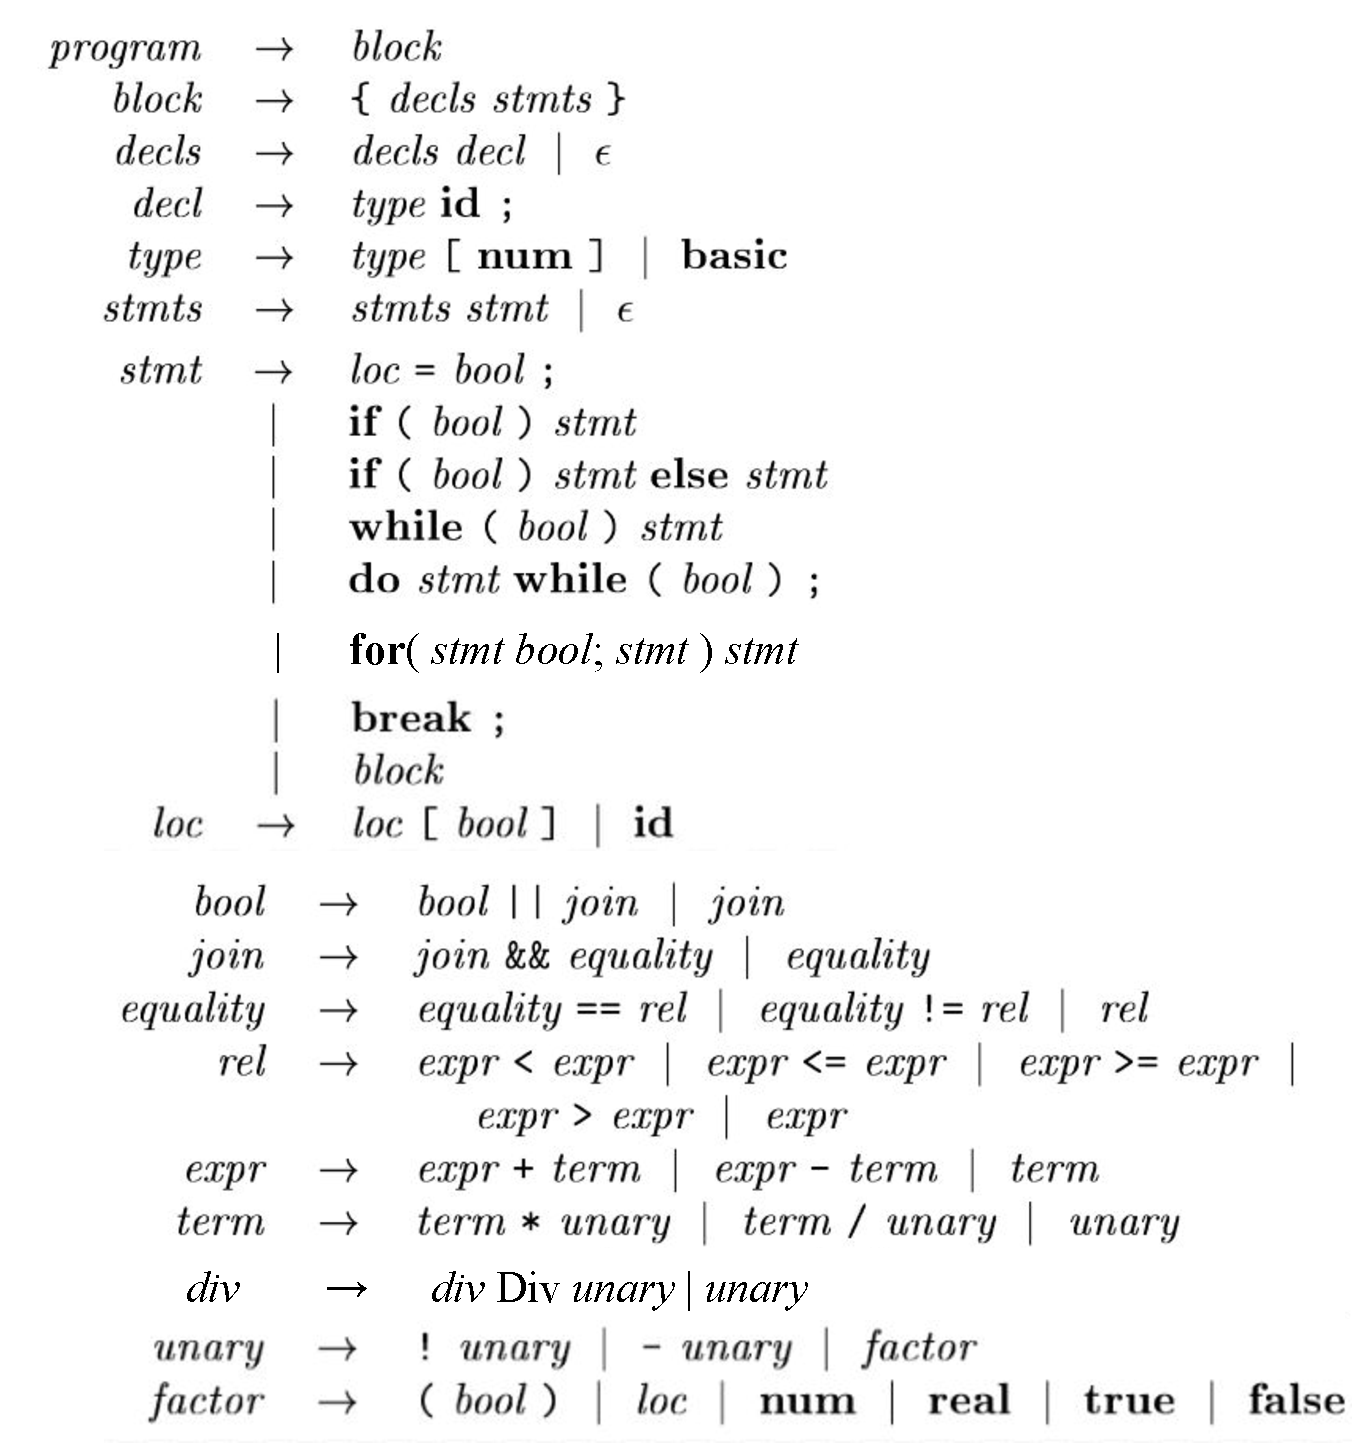
\includegraphics[scale=0.5]{grammar.pdf}
        \label{fig_3a}
    \end{figure}

\end{solution}
\noindent\rule{7in}{2.8pt}
%%%%%%%%%%%%%%

%%%%%%%%%%%%%%%%%%%%%%%%%%%%%%%%%%%%%%%%%%%%%%%%%%%%%%%%%%%%%%%%%%%%%%%%%
% Deliverables
%%%%%%%%%%%%%%%%%%%%%%%%%%%%%%%%%%%%%%%%%%%%%%%%%%%%%%%%%%%%%%%%%%%%%%%%%%%%%%%%%%%%%%%%%%%%%%%%%%%%%%%%%%%%%%%%%%%%%%%%%%%%%%%%%%%%%%%%
\bf{Deliverables:} A zip file containing
\begin{itemize}
    \item All folders from the dragon-front-source file you were given, plus your changes
    \item A text file containing a simple list of all changes you made to the source files, clearly labeled
    \item A pdf file with relevant answers to questions in this document.
    \item A text file marked readme that contains:
          \begin{itemize}
              \item Full name and Case ID
              \item (not required) any special notes about your implementation the grader should be aware of
          \end{itemize}
\end{itemize}

\noindent\rule{7in}{2.8pt}
Tip: An app such as Notepad++ can be used to create .t files which you can use to test your program in the test folder.
\end{document}
